\subsection{Vue d'ensemble et système de coordonnées}\label{chapter-LHC-section-CMS-subsec-overview_and_coordinates}
Le détecteur CMS est installé dans la caverne du point d'interaction numéro~5 du LHC, visible sur la figure~\ref{fig-CERN_map} au Nord de l'installation, dans la commune de Cessy, en France.
Il a été conçu avec pour but premier l'étude de la brisure de symétrie électrofaible et la recherche du boson de Higgs~\cite{cms_letter_intent}.
Son design généraliste permet de l'utiliser pour de nombreuses autres analyses de physique, allant de mesures de précision à la recherche d'une nouvelle physique.
Les collisions d'ions lourds réalisées au LHC peuvent également être étudiées grâce à ce détecteur.
\par La figure~\ref{fig-chapter-LHC-section-CMS-subsec-overview_and_coordinates-vue_eclatee_CMS} présente une vue éclatée du détecteur CMS.
Il possède une forme cylindrique de \SI{28.7}{\meter} de long et \SI{15}{\meter} de diamètre pour un poids total de \num{14000} tonnes.
Il est structuré en couches concentriques, chacune ayant un rôle spécifique détaillé dans les sections qui suivent.
À partir du centre du détecteur, lieu des collisions, se trouvent dans l'ordre
le trajectographe,
le calorimètre électronique,
le calorimètre hadronique,
le solénoïde donnant son \og S \fg{} à CMS et
les chambres à muons donnant son \og M \fg{} à CMS, encastrées dans la culasse de fer.
Des calorimètres avancés se trouvent aux extrémité du détecteur le long de l'axe du faisceau.
Le détecteur propose ainsi une couverture d'un angle solide de presque $4\pi\usp\SI{}{\steradian}$, \ie\ de presque toutes les directions, ce qui est capital afin de reconstruire les collisions.
\begin{figure}[t]
\centering
\includegraphics[width=\textwidth]{\PhDthesisdir/plots_and_images/CMS_slices/from_CMS_document_13631-v4/cms_160312_06-FR.tex}
\caption[Vue éclatée du détecteur CMS.]{Vue éclatée du détecteur CMS~\cite{CMS_document_13631-v4}.}
\label{fig-chapter-LHC-section-CMS-subsec-overview_and_coordinates-vue_eclatee_CMS}
\end{figure}
\par L'acronyme CMS signifie ainsi \emph{Compact Muon Solenoïd}, \ie\ Solénoïde Compact à Muons.
Son qualificatif de \og compact \fg{} se comprend par comparaison à d'autres détecteurs de physique des particules, comme son homologue au LHC, ATLAS.
Ce détecteur est également cylindrique et fait \SI{40}{\meter} de long pour \SI{22}{\meter} de diamètre, soit un volume trois fois plus grand que celui de CMS.
Pourtant, ATLAS ne pèse \og que \fg{} \num{7000} tonnes, deux fois moins que CMS.
Il n'y a en effet que peu d'espace vide dans le volume occupé par le détecteur CMS.
\par La géométrie cylindrique du détecteur pousse à définir un système de coordonnées également cylindrique en complément d'un repère cartésien.
Le schéma de la figure~\ref{fig-chapter-LHC-section-CMS-subsec-overview_and_coordinates-CMS_3D_phi_theta_defs} illustre la définition de ces systèmes de coordonnées.
L'origine $O$ des repères est le centre du détecteur où les protons entrent en collision.
L'axe \axis{x} pointe vers le centre du LHC, l'axe \axis{y} vers le haut ($\vec{g}\cdot\bvec_y<0$) et l'axe \axis{z} est aligné avec le faisceau tel que $(\bvec_x, \bvec_y, \bvec_z)$ forme un trièdre direct.
Le système de coordonnées cylindriques est défini par la distance à l'origine et deux angles $\theta\in[0,\pi]$ et $\phi\in[-\pi,\pi]$.
L'angle entre les plans $(\bvec_x, \bvec_z)$ et $(\vec{a}, \bvec_z)$ est $\phi$, défini dans le plan $(\bvec_y,\bvec_z)$ à partir de l'axe \axis{x}.
L'angle entre les directions $\vec{a}$ et $\bvec_z$ est $\theta$.
\begin{figure}[h]
\centering
{\tdplotsetmaincoords{70}{115}
\tdplotsetrotatedcoords{-90}{-90}{-90}
\begin{tikzpicture}[tdplot_rotated_coords,scale=1.25]
%% base
\draw [->] (0,0,-3)--(0,0,3) node[above] {$\bvec_z$};
\draw [->] (0,0,0)--(1,0,0) node[above] {$\bvec_x$};
\draw [->] (0,0,0)--(0,1,0) node[above] {$\bvec_y$};

%% CMS barrel
\draw (0,0,-2.1) circle (1.5);
\draw (0,0,2.1) circle (1.5);
\def\CMSphiangle{70}
\draw ({1.5*cos(\CMSphiangle)},{1.5*sin(\CMSphiangle)},-2.1) --+(0,0,4.2);
\draw ({1.5*cos(180+\CMSphiangle)},{1.5*sin(180+\CMSphiangle)},-2.1) --+(0,0,4.2);

%% beam
%\draw [ltcolorred, very thick, -latex] (0,0,-2)--(0,0,0);
%\draw [ltcolorred, very thick, -latex] (0,0,2)--(0,0,0);
%% particule sortante
\draw [ltcolorblue, thick, -latex] (0,0,0)--(1.5,1.5,{1.5*2^0.5}) node [right] {$\vec{a}$};
%% vertex primaire
%\fill [ltcolororange] (0,0,0) circle (2pt);

%% track plane
\def\CMSphiangle{45}
\draw [densely dotted] ({1.5*cos(\CMSphiangle)},{1.5*sin(\CMSphiangle)},-2.1) -- ({1.5*cos(\CMSphiangle)},{1.5*sin(\CMSphiangle)},2.1) -- ({-1.5*cos(\CMSphiangle)},{-1.5*sin(\CMSphiangle)},2.1) -- ({-1.5*cos(\CMSphiangle)},{-1.5*sin(\CMSphiangle)},-2.1) --({1.5*cos(\CMSphiangle)},{1.5*sin(\CMSphiangle)},-2.1);

%% phi angle
\draw [densely dotted] (0,0,2.1)--(1.5,0,2.1);
\draw [-latex] (1,0,2.1) arc (0:45:1);
\draw (.75,.25,2.1) node {$\phi$};

%% theta angle
\tdplotsetrotatedcoords{0}{45}{90}
%\draw [tdplot_rotated_coords, ltcolorgreen,<->] (-2.1,1.5,0)--(2.1,-1.5,0);
%\draw [tdplot_rotated_coords, ltcolorgreen,<->] (-2.1,-1.5,0)--(2.1,1.5,0);
%\draw [tdplot_rotated_coords, ltcolorcyan,<->] (-1.5,2.1,0)--(1.5,-2.1,0);
%\draw [tdplot_rotated_coords, ltcolorcyan,<->] (-1.5,-2.1,0)--(1.5,2.1,0);
\draw [tdplot_rotated_coords,-latex] (1,0,0) arc (0:45:1);
\draw [tdplot_rotated_coords] (22.5:1.2) node {$\theta$};

%% origin
\fill (0,0,0) circle (2pt);
\draw (0,0,0) node [below left] {$O$};
\end{tikzpicture}}
\caption[Système de coordonnées du détecteur CMS.]{Système de coordonnées du détecteur CMS. L'axe \axis{x} pointe vers le centre du LHC, l'axe \axis{y} vers le haut ($\vec{g}\cdot\bvec_y<0$) et l'axe \axis{z} est aligné avec le faisceau tel que $(\bvec_x, \bvec_y, \bvec_z)$ forme un trièdre direct. L'angle entre les plans $(\bvec_x, \bvec_z)$ et $(\vec{a}, \bvec_z)$ est $\phi$, défini dans le plan $(\bvec_y,\bvec_z)$ à partir de l'axe \axis{x}. L'angle entre les directions $\vec{a}$ et $\bvec_z$ est $\theta$.}
\label{fig-chapter-LHC-section-CMS-subsec-overview_and_coordinates-CMS_3D_phi_theta_defs}
%\end{figure}
%\begin{figure}[h]
%\centering
\vspace{\baselineskip}

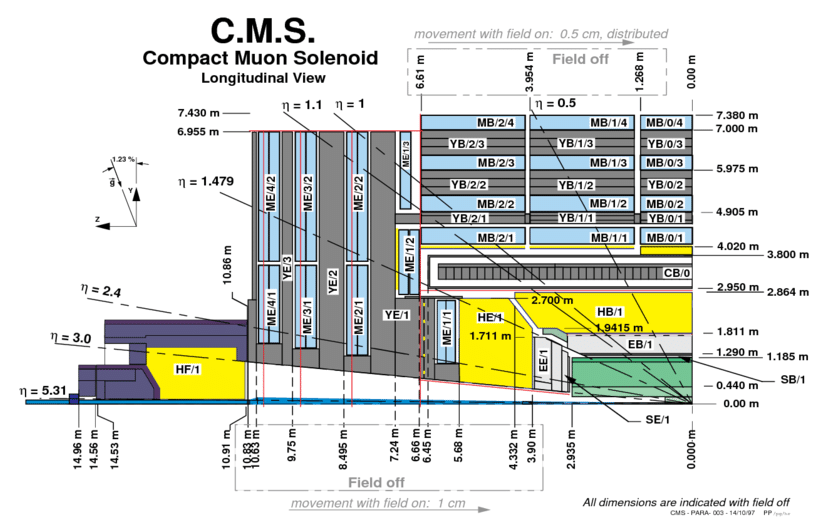
\includegraphics[width=\textwidth]{\PhDthesisdir/plots_and_images/from_CMS_alignment_photodetectors/CMS-eta-ranges.png}
\caption[Vue longitudinale d'un quadrant du détecteur CMS.]{Vue longitudinale d'un quadrant du détecteur CMS~\cite{CMS_alignment_photodetectors}. Les directions correspondant à quelques valeurs de pseudo-rapidité sont illustrées et des mesures de distances par rapport au centre du détecteur, lieu des collisions, sont indiquées. Le sol de la caverne présente une inclinaison de \SI{1.23}{\%} par rapport à la direction de la gravité locale $\vec{g}$, ce que montre le schéma à gauche.}
\label{fig-chapter-LHC-section-CMS-subsec-overview_and_coordinates-CMS-eta-ranges}
\end{figure}
\par L'angle $\theta$ n'est généralement pas utilisé directement et est remplacé par la \og pseudo-rapidité \fg{} $\eta$ définie comme
\begin{equation}
\eta = - \ln(\tan(\frac{\theta}{2}))
\mend
\label{eq-chapter-LHC-section-CMS-subsec-overview_and_coordinates-eta_definition}
\end{equation}
La pseudo-rapidité est ainsi égale à zéro dans le plan transverse, \ie\ le plan \plane{x}{y}.
L'usage de cette variable est motivé par la densité de production de particules qui est constante suivant $\eta$ et non selon $\theta$.
De plus, dans la limite \og ultra-relativiste \fg{} \ie\ $\abs{\vec{p}}\gg m$, condition remplie au LHC, la pseudo-rapidité tend vers la rapidité $y$ (à ne pas confondre avec la coordonnée $y$) des particules,
\begin{equation}
y = \frac{1}{2} \ln(\frac{E+p_zc}{E-p_zc})
\mend
\end{equation}
Or la rapidité est un invariant de Lorentz, ainsi au LHC $\eta$ est en très bonne approximation un invariant de Lorentz, contrairement à $\theta$.
La figure~\ref{fig-chapter-LHC-section-CMS-subsec-overview_and_coordinates-CMS-eta-ranges} présente un quadrant du détecteur CMS sur lequel figurent quelques valeurs de pseudo-rapidité est les directions correspondantes dans le plan \plane{y}{z}.
\par Du fait de la structure des protons discutée dans la section~\ref{chapter-LHC-section-LHC-subsec-pp_collisions}, lors de la collision, l'impulsion totale selon l'axe des faisceaux est inconnue.
Seule l'impulsion totale dans le plan transverse, \ie\ le plan \plane{x}{y}, est nulle.
C'est pourquoi des variables relatives au plan transverse sont définies, en particulier l'impulsion transverse \vpT, sa norme \pT\ et l'énergie transverse \ET,
\begin{equation}
\vpT = p_x\bvec_x + p_y\bvec_y
\msep
\pT = \sqrt{p_x^2+p_y^2}
\msep
\ET = E\sin\theta = \frac{E}{\cosh\eta}
\mend
\end{equation}